\documentclass[./CGMPortfolio.tex]{subfiles}\providecommand{\econtexRoot}{}
\renewcommand{\econtexRoot}{.}

% Different execution depending on whether compiling main file or as standalone subfile
\onlyinsubfile{\externaldocument{CGMPortfolio}} % Get xrefs -- esp to appendix 
%-- from main file; only works properly if main file has already been compiled; 
%order: Compile this file, then main, then this one again
\begin{document}

\hfill{\tiny \texname.tex, \today}

\begin{verbatimwrite}{CGMPortfolio.title}  % Write title to .title file
Cocco, Gomes, and Maenhout (2005) REMARK
\end{verbatimwrite}

\title{Cocco, Gomes, and Maenhout (2005) \\ REMARK}

\author{Mateo Vel\'asquez-Giraldo \and Matthew V. Zahn}

\keywords{Lifecycle, Portfolio Choice, Replication}

\maketitle 

\hypertarget{abstract}{}
\begin{abstract}
This paper contains the highlights from the REMARK file in Code>Python folder.
\end{abstract}

% Various resources 
\hypertarget{links}{}
\begin{small}
\parbox{\textwidth}{
\begin{center}
\begin{tabbing}
\texttt{~Archive:~} \= \= \url{http://econ.jhu.edu/people/ccarroll/BufferStockTheory.zip} \kill \\  %
\texttt{~~GitHub:~} \> \> 
\url{http://github.com/econ-ark/REMARK/REMARKS/CGMPortfolio} \\
\texttt{~~~~~~~~~~} \> \> \textit{(In GitHub repo, see \texttt{/Code} for tools for solving and simulating the model)} \\
\end{tabbing}
\end{center}
          
\href{https://mybinder.org/v2/gh/matthew-zahn/CGMPort/develop?filepath=REMARK\%2FCGM_REMARK.ipynb}{CLICK HERE} for an interactive \href{https://en.wikipedia.org/wiki/Project\_Jupyter\#Jupyter_Notebook}{Jupyter Notebook} that uses the \href{https://econ-ark/HARK}{Econ-ARK/HARK} toolkit to produce our figures (warning: it may take several minutes to launch).  Information about citing the toolkit can be found at \href{https://econ-ark.org/acknowledging/}{Acknowleding Econ-ARK}.
} % end parbox{\textwidth}
\end{small}

\begin{authorsinfo}
\name{Contact: \href{mailto:mvelasq2@jhu.edu}{\texttt{mvelasq2@jhu.edu}}, \href{mailto:matthew.zahn@jhu.edu}{\texttt{matthew.zahn@jhu.edu}}, Department of Economics, 590 Wyman Hall, Johns Hopkins University, Baltimore, MD 21218, \url{https://t.co/uaflostQyF?amp=1}, \url{http://matthewvzahn.com}.}
\end{authorsinfo}

\thanks{All numerical results herein were produced using the \href{https://econ-ark/HARK}{Econ-ARK/HARK} toolkit; for further reference options see \href{https://econ-ark.org/acknowledging/}{Acknowleding Econ-ARK}.  Thanks to Chris Carroll and Sylvain Catherine for comments and guidance.}

\titlepagefinish

\newtheorem{defn}{Definition}
\newtheorem{theorem}{Theorem}

\hypertarget{Introduction}{}
\section{Introduction}

This exercise uses the \href{https://github.com/econ-ark/hark}{Econ-ARK/HARK} 
toolkit to attempt a replication of \cite{cgm2015}'s main results. The main 
HARK tool used 
here is the $\texttt{PortfolioConsumerType}$ 
class. For an introduction to this module, see the 
\href{https://hark.readthedocs.io/en/latest/}{HARK's 
	Documentation}.

Our results using the HARK toolkit resemble those of the original paper, but we 
have not been able to replicate its results exactly for reasons that we have 
not been able to track down. We suspect there might be subtleties in the 
normalization or calibration that we have missed and that could be causing the 
discrepancies. We would be thankful if a reader (or the original authors) were 
able to discover the reason for the discrepancies, and could issue a pull 
request for a revision that reconciles them.

We thank Chris Carroll and Sylvain Catherine for comments and guidance.

\hypertarget{The-base-model}{}
\section{The base model}

\cite{cgm2015}' aim is to represent the life cycle of a consumer that is 
exposed to uninsurable labor income risk and how he chooses to allocate his 
savings between a risky and a safe asset, without the possibility to borrow or 
short-sell.

\subsection{Dynamic problem}

The problem of an agent $i$ of age $t$ in the base model is recursively represented as

\begin{verbatimwrite}{\EqDir/DynProb.tex}
	\begin{align}
		V_{i,t} =& \max_{0\leq C_{i,t} \leq X_{i,t}, \alpha_{i,t}\in[0,1]} U(C_{i,t}) + \delta p_t E_t\{ V_{i,t+1} (X_{i,t+1}) \}\\
		&\text{s.t} \nonumber \\
		&X_{i,t+1} = Y_{i,t+1} + (X_{i,t} - C_{i,t})(\alpha_{i,t} R_{t+1} + (1-\alpha_{i,t})\bar{R}_f)
	\end{align}
\end{verbatimwrite}
	\begin{align}
		V_{i,t} =& \max_{0\leq C_{i,t} \leq X_{i,t}, \alpha_{i,t}\in[0,1]} U(C_{i,t}) + \delta p_t E_t\{ V_{i,t+1} (X_{i,t+1}) \}\\
		&\text{s.t} \nonumber \\
		&X_{i,t+1} = Y_{i,t+1} + (X_{i,t} - C_{i,t})(\alpha_{i,t} R_{t+1} + (1-\alpha_{i,t})\bar{R}_f)
	\end{align}

where $C_{i,t}$ is consumption, $\alpha_{i,t}$ is the share of savings 
allocated to the risky asset, $Y_{i,t}$ is labor income, and $X_{i,t}$ 
represents wealth. The utility function $U(\cdot)$ is assumed to be CRRA in the 
base model. Extensions beyond the baseline model include an additively 
separable bequest motive in the utility function. The discount factor is 
$\delta$ and $p_t$ is the probability of survival from $t$ to $t+1$. Death is 
certain at a maximum period $T$.

Note that the consumer cannot borrow or short-sell.

The control variables in the problem are $\{C_{it}, \alpha_{it}\}^T_{t=1}$ and the state variables are $\{t, X_{it}, v_{it} \}^T_{t=1}$. The agent solves for  policy rules as a function of the state variables\textemdash $C_{it}(X_{it}, v_{it})$ and $\alpha_{it}(X_{it}, v_{it})$.

\subsection{Labor income}

An important driver of the paper's results is the labor income process. It is 
specified as follows:
\begin{equation}
\log Y_{i,t} = f(t,Z_{i,t}) + v_{i,t} + \epsilon_{i,t}, \quad \text{for } t\leq K.
\end{equation}
where $K$ is the (exogenous) age of retirement, $Z_{i,t}$ are demographic 
characteristics, $\epsilon_{i,t}\sim \mathcal{N}(0,\sigma^2_\epsilon)$ is a 
transitory shock, and  $v_{i,t}$ is a permanent component following a random 
walk
\begin{equation}
v_{i,t} = v_{i,t-1} + u_{i,t} = v_{i,t-1} + \xi_t + \omega_{i,t}
\end{equation}
in which the innovation is decomposed into an aggregate ($\xi_t$) and an 
idiosyncratic component ($\omega_{i,t}$), both following mean-0 normal 
distributions.

Post-retirement income is a constant fraction $\lambda$ of permanent income in the last working year $K$.

A crucial aspect of the labor income process is that $f(\cdot,\cdot)$ is calibrated to match income profiles in the PSID, capturing the usual humped shape of income across lifetime.

\subsection{Matching labor income in HARK}

In HARK's consumption-saving models, the income process takes the form
\begin{equation}
\ln Y_t = \ln P_t + \ln \theta_t
\end{equation}
where $P_t$ represents permanent income and $\ln \theta_t \sim N(0,\sigma_\theta)$ transitory shocks to income. Permanent income evolves according to
\begin{equation}
\ln P_{t+1} = \ln \Gamma_{t+1} +  \ln \psi_{t+1} + \ln P_t
\end{equation}
where $\Gamma_{t+1}$ is a deterministic growth factor, and $\ln \psi_{t+1} \sim N(0,\sigma_\psi)$ a permanent income shock. 


To represent the author's assumptions in HARK, we express both income processes as sums of deterministic components and i.i.d shocks
\begin{align}
\text{Cocco et. al} &\quad& \ln Y_{i,t} &=& f(t,Z_{i,t}) + v_{i,0} &+&\sum_{k=1}^t u_{i,k} &+&\qquad \varepsilon_{i,t} \\
\text{HARK}        &\quad& \ln Y_{i,t} &=& \ln P_{i,0} + \sum_{k=1}^t \ln \Gamma_k &+&\sum_{k=1}^t \ln \psi_{i,k} &+& \qquad \ln \theta_{i,t}.
\end{align}

These representations make evident the mapping that we use
\begin{table}[h]
\centering
\caption{Mapping to HARK}
\label{tab:Mapping}
\begin{tabular}{|c|c|}
\hline
\textbf{HARK} & \textbf{Cocco et. al} \\ \hline
$\ln$ $P_{i,0}$ & $f(0,Z_{i,0})$ + $v_{i,0}$ \\ \hline
$\ln$ $\Gamma_{t+1}$ & $f(t+1$, $Z_{i,t+1})$ - $f(t,Z_{i,t})$ \\ \hline
$\ln$ $\psi_{i,k}$ & $u_{i,k}$ \\ \hline
$\ln$ $\theta_{i,t}$ & $\varepsilon_{i,t}$ \\ \hline
$\ln$ $\psi_{i,k}$ & $u_{i,k}$ \\ \hline
$\ln$ $\theta_{i,t}$ & $\varepsilon_{i,t}$ \\ \hline
\end{tabular}
\end{table}

and to achieve a retirement income that is equal to a fraction $\lambda$ of 
permanent income in the last working period $K$, we simply make $\Gamma_{K+1} = 
\lambda$ and $\Gamma_{t} = 1$ $\forall t>K+1$.

\subsection{Assets and their returns}

There are two assets available for consumers to allocate their savings.
\begin{itemize}
	\item Bonds: paying a risk-free return $\bar{R}_f$.

	\item Stocks: paying a stochastic return $R_t = \bar{R}_f + \mu + \eta_t$, where the stochastic component $\eta_t \sim \mathcal{N}(0, \sigma^2_\eta)$ is allowed to be correlated with the aggregate labor income innovation $\xi_t$.
	
\end{itemize}

The borrowing and short-selling constraints ensure that agents cannot allocate negative dollars to either of these assets or borrow against future labor income or retirement wealth. Recall $\alpha_{i,t}$ is the proportion of the investor's savings that are invested in the risky asset. The model's constraints imply that $\alpha_{i,t}\in[0,1]$ and wealth is non-negative.

\hypertarget{Calibration}{}
\section{Calibration\textemdash Summary}

The paper defines and calibrates several parameters which are summarized in Table \ref{tab:Calibration}:

\begin{table}
\begin{center}\renewcommand{\arraystretch}{1.5}
\caption{Microeconomic Model Calibration}\label{table:Calibration}
\begin{tabular}{|c|ccl|c|}
\hline
\multicolumn{5}{|l|}{Calibrated Parameters}  \\ \hline
Description                     & \multicolumn{1}{c}{Parameter} & Value & \multicolumn{2}{c|}{Source}\\ \hline
Permanent Income Growth Factor  & \multicolumn{1}{c}{$\PGro$} & 1.03 & \multicolumn{2}{c|}{PSID: Carroll (1992)} \\
Interest Factor                 & \multicolumn{1}{c}{$\Rfree$} & 1.04 & \multicolumn{2}{c|}{Conventional} \\
Time Preference Factor          & \multicolumn{1}{c}{$\beta$} & 0.96 & \multicolumn{2}{c|}{Conventional} \\
Coefficient of Relative Risk Aversion & \multicolumn{1}{c}{$\CRRA$} & 2 & \multicolumn{2}{c|}{Conventional} \\
Probability of Zero Income      & \multicolumn{1}{c}{$\pZero$} & 0.005 & \multicolumn{2}{c|}{PSID: Carroll (1992)} \\
Std Dev of Log Permanent Shock  & \multicolumn{1}{c}{$\sigma_{\pshk}$} & 0.1 & \multicolumn{2}{c|}{PSID: Carroll (1992)} \\
Std Dev of Log Transitory Shock & \multicolumn{1}{c}{$\sigma_{\theta}$} & 0.1 & \multicolumn{2}{c|}{PSID: Carroll (1992)} \\ \hline
\end{tabular}
\end{center}
\end{table}
\begin{table}
\begin{center}\renewcommand{\arraystretch}{1.5}
\caption{Model Characteristics Calculated from Parameters}\label{table:Calibration}
\begin{tabular}{|c|ccl|c|}
\hline
%\multicolumn{5}{|l|}{Model Characteristics Calculated From Parameters}  \\ \hline
                                            & \multicolumn{3}{c|}{}                                      & Approximate \\
                                            & \multicolumn{3}{c|}{}                                       & Calculated \\
Description                                 & \multicolumn{3}{c|}{Symbol and Formula}                       & Value \\ \hline
Finite Human Wealth Measure                 & $\Rnorm^{-1}$ & $\equiv$ & $\PGro/\Rfree$                    & 0.990 \\
PF Finite Value of Autarky Measure& $\beth$ & $\equiv$ & $\beta \PGro^{1-\CRRA}$                    & 0.932 \\
Growth Compensated Permanent Shock            & $\InvEpShkInv $ & $\equiv$ & $ (\EpShkInv)^{-1}$               & 0.990 \\
Uncertainty-Adjusted Growth                 & $\PGroAdj $ & $\equiv$ & $ \PGro \InvEpShkInv$        & 1.020 \\
Utility Compensated Permanent Shock                & $\uInvEpShkuInv $ & $\equiv$ & $ (\Ex_{t}[\pShk^{1-\CRRA}])^{1/(1-\CRRA)}$ & 0.990 \\
Utility Compensated Growth                     & $\PGrouAdj $ & $\equiv$ & $ \PGro \uInvEpShkuInv$        & 1.020 \\
Absolute Patience Factor                    & $\Pat_{\phantom{\Rfree}} $ & $\equiv$ & $ (\Rfree \beta)^{1/\CRRA}$                & 0.999 \\
Return Patience Factor                      & $\PatR$ & $\equiv$ & $\Pat/\Rfree $     & 0.961 \\
PF Growth Patience Factor    & $\PatPGro$ & $\equiv$ & $\Pat/\PGro $      & 0.970 \\
Growth Patience Factor                      & $\PatPGroAdj$ & $\equiv$ & $ \Pat/\PGroAdj$& 0.980 \\
Finite Value of Autarky Measure         & $\DiscAltuAdj $ & $\equiv$ & $ \beta \PGro^{1-\CRRA}\uInvEpShkuInv^{1-\CRRA}$       & 0.941 \\ \hline
\end{tabular}
\end{center}
\end{table}


\hypertarget{Normalization}{}
\section{A note on normalization}

The problem as specified above makes the value function homogeneous with respect to permanent labor income. This is convenient as it allows for a re-statement of the problem in variables that are normalized by permanent income or its random components, eliminating a state variable.

The authors report (page 497) taking the normalization $v_{i,t} = 1$. This amounts to defining normalized variables $\tilde{\cdot}$ as the original variable divided by $e^{v_{i,t}-1}$. For instance:

\begin{equation}
\tilde{Y_{i,t}} = \frac{Y_{i,t}}{\exp(v_{i,t}-1)} = \frac{\exp (f(t,Z_{i,t}) + v_{i,t} + \varepsilon_{i,t})}{\exp(v_{i,t}-1)} = \exp( f(t,Z_{i,t}) + 1 + \varepsilon_{i,t} )
\end{equation}

These normalized variables have the convenient interpretation of the state that things would be in if, it weren't for permanent shocks. The author's depictions of policy functions are presented in terms of these normalized variables.

On the other hand, HARK normalizes the problem by total permanent income $P_t = \exp (f(t,Z_{i,t}) + v_{i,t})$ and its solution objects are therefore in terms of normalized variables $\hat{\cdot}$, defined as
\begin{equation}
\hat{X_{i,t}} = \frac{X_{i,t}}{P_{i,t}} = \frac{X_{i,t}}{\exp (f(t,Z_{i,t}) + v_{i,t})}.
\end{equation}

Therefore, to present our results in a way consistent with that of the original authors, we would use the following relationship
\begin{equation}
\tilde{X_{i,t}} = \hat{X_{i,t}} \times \exp (f(t,Z_{i,t})+1)
\end{equation}

However, our results are much more consistent with those of the original authors when we take the normalization $v_{i,t} = 0$, which also make sense since it makes the random-walk multiplicative part of permanent income $\exp{v_{i,t}}=1$. We therefore assume this is a typo, take $v_{i,t} = 0$, document this issue in Section \ref{sec:Puzzles} below, and use the relationship
\begin{equation}
\tilde{X_{i,t}} = \hat{X_{i,t}} \times \exp (f(t,Z_{i,t})).
\end{equation}

\hypertarget{Key-Results}{}
\section{Key Results}

\subsection{The optimal risky asset share}

Figure \ref{fig:RSharePol} shows the policy function for the risky portfolio share as a function of wealth at different ages.

The optimal risky share is decreasing in wealth. The authors argue this is due to the fact that, at low levels of wealth, relatively safe human wealth represents a higher fraction of the consumer's wealth, so he shifts his tradeable wealth towards riskier alternatives.

Analyzing the policy rule by age also shows that the risky share increases from young to middle age, and decreases from middle to old age. This is consistent with the previous interpretation: shares trace the humped shape of labor earnings.

These estimates are different from what is produced in the original paper, which are also reproduced below. Generally, the policy functions do not share the same curvature, which leads to greater reductions in the optimal portfolio share at lower levels of wealth.

\providecommand{\figName}{Risky-Share-Policy-Function} % Allows generic definition of hypertargets based on title of figure
\providecommand{\figFile}{RShare_Pol} %  and on filename
\hypertarget{\figFile}{}
\hypertarget{\figName}{}
\begin{figure}[]
	\centerline{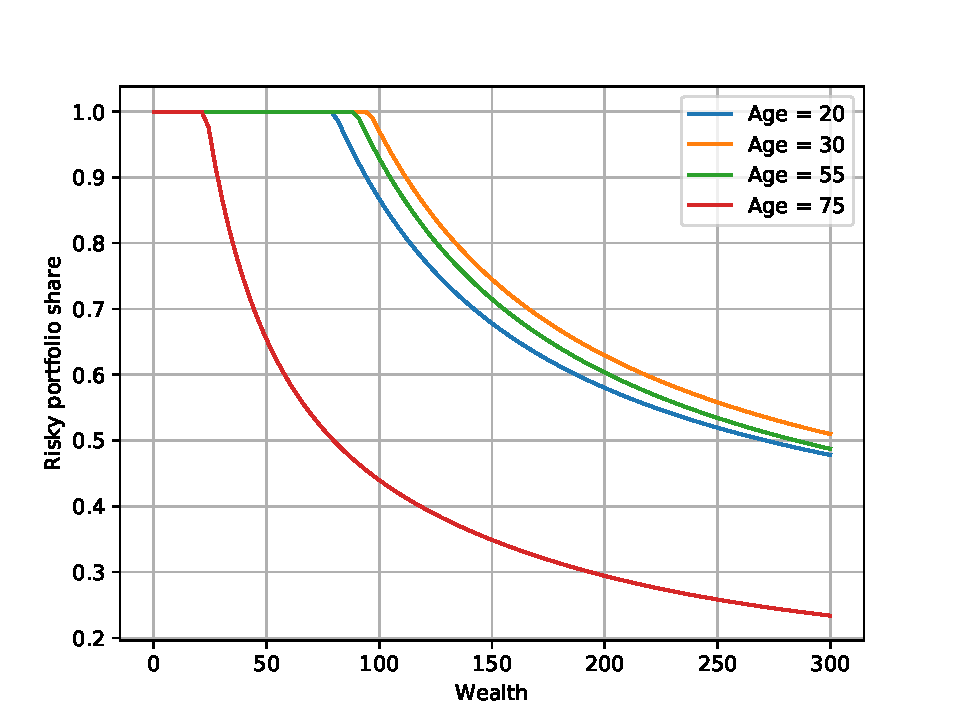
\includegraphics[width=6in]{\econtexRoot/\FigsRaw/RShare_Pol}}
	\caption{Risky Share Policy Function}
	\label{fig:RSharePol}
\end{figure}
 % Read in the tex to generate the figure

\subsection{Consumption behavior}

Figure \ref{fig:cPolFunc} below shows the policy function for consumption as a function of wealth at different ages.

At all age levels consumption increases with wealth. The consumption function also appears to shift upwards as life progresses.

Our consumption policy functions again do not match those of the original paper, which are also reproduced below. Consumption also appears to increase with age in our policy functions that does not come through in the results presented in the paper. 

\providecommand{\figName}{Consumption-Policy-Function} % Allows generic definition of hypertargets based on title of figure
\providecommand{\figFile}{Cons_Pol} %  and on filename
\hypertarget{\figFile}{}
\hypertarget{\figName}{}
\begin{figure}[]
	\centerline{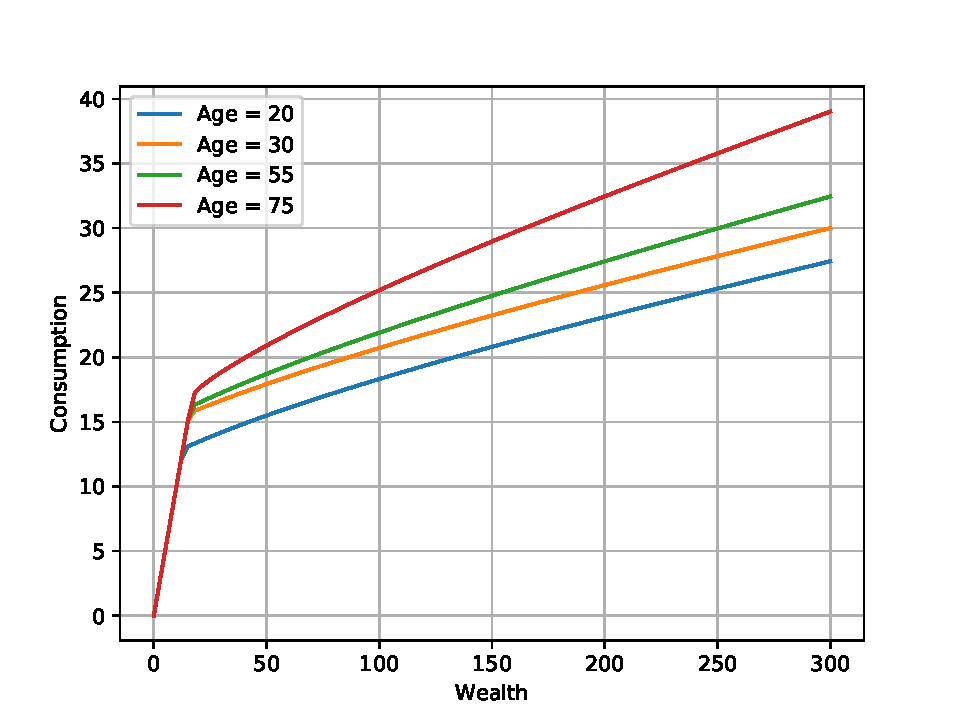
\includegraphics[width=6in]{\econtexRoot/\FigsRaw/Cons_Pol}}
	\caption{Consumption Policy Function}
	\label{fig:cPolFunc}
\end{figure}
 % Read in the tex to generate the figure

\hypertarget{Simulations}{}
\section{Simulations}

Using the policy functions obtained from solving the model we present a series of simulations to highlight features of the model.

We first run a few simulations to verify the quality of our calibration.

The Figures \ref{fig:YSim} and \ref{fig:RShareSim} below show simulated levels of permanent income and risky portfolio shares for 5 agents over their life spans. We can see the model generates a heterogeneous permanent income distribution. Interestingly, all of these agents tend to follow the same general pattern for investing in the risky asset. Early in life, all of their portfolios are invested in the risky asset. This declines as the agent ages and converges to approximately 35\% once they reach retirement.

\providecommand{\figName}{Income-Simulation} % Allows generic definition of hypertargets based on title of figure
\providecommand{\figFile}{Y_Sim} %  and on filename
\hypertarget{\figFile}{}
\hypertarget{\figName}{}
\begin{figure}[]
	\centerline{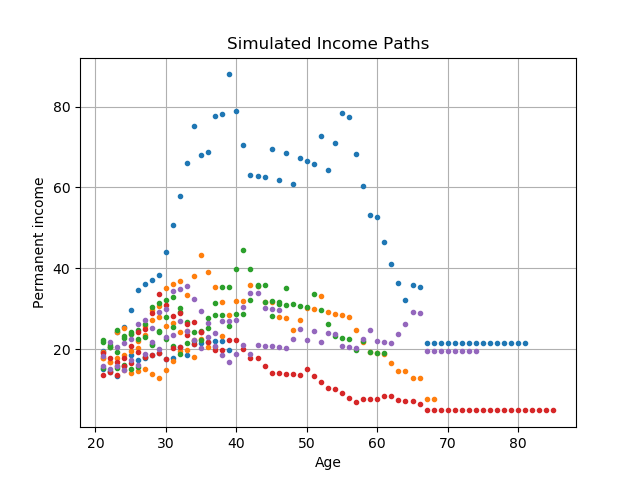
\includegraphics[width=6in]{\econtexRoot/\FigsRaw/Y_Sim}}
	\caption{Income Simulation}
	\label{fig:YSim}
\end{figure}
 % Read in the tex to generate the figure

\providecommand{\figName}{Risky-Share-Simulation} % Allows generic definition of hypertargets based on title of figure
\providecommand{\figFile}{RShare_Sim} %  and on filename
\hypertarget{\figFile}{}
\hypertarget{\figName}{}
\begin{figure}[h]
	\centerline{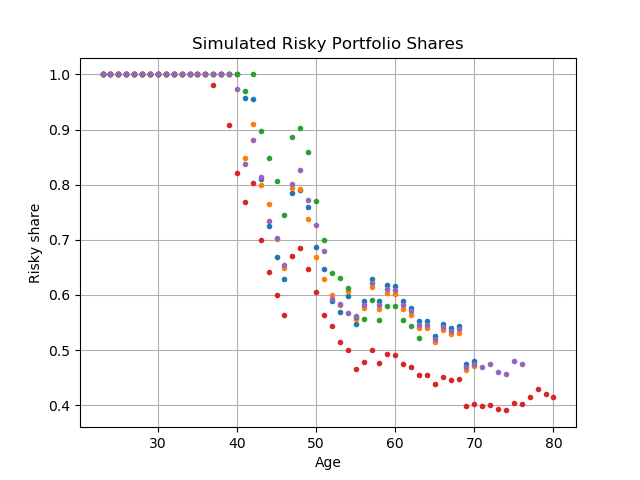
\includegraphics[width=6in]{\econtexRoot/\FigsRaw/RShare_Sim}}
	\caption{Risky Share Simulation}
	\label{fig:RShareSim}
\end{figure}
 % Read in the tex to generate the figure

\subsection{The average life cycle patterns}

We now increase the number of simulations to examine and compare the behavior of the mean values of variables of interest at different ages, conditional on survival. In each case we present the original plots from the paper for reference.

Figure \ref{fig:YMC} below illustrates the average dynamics of permanent income, consumption, and market resources across all of the simulated agents. The plot follows the general pattern observed in the original paper. However, our results show that the agents are accumulating significantly more market resources. Figure \ref{fig:RShareMean} presents mean portfolio share conditional on survival.

\providecommand{\figName}{Variable-Means-Conditional-on-Survival} % Allows generic definition of hypertargets based on title of figure
\providecommand{\figFile}{YMC_Means} %  and on filename
\hypertarget{\figFile}{}
\hypertarget{\figName}{}
\begin{figure}[]
	\centerline{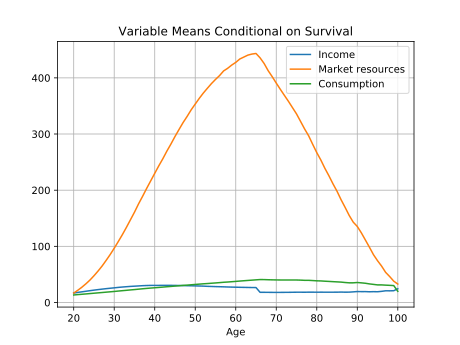
\includegraphics[width=6in]{\econtexRoot/\FigsRaw/YMC_Means}}
	\caption{Variable Means Conditional on Survival}
	\label{fig:YMC}
\end{figure}
 % Read in the tex to generate the figure

\providecommand{\figName}{RShare-Means-Conditional-on-Survival} % Allows generic definition of hypertargets based on title of figure
\providecommand{\figFile}{RShare_Means} %  and on filename
\hypertarget{\figFile}{}
\hypertarget{\figName}{}
\begin{figure}[]
	\centerline{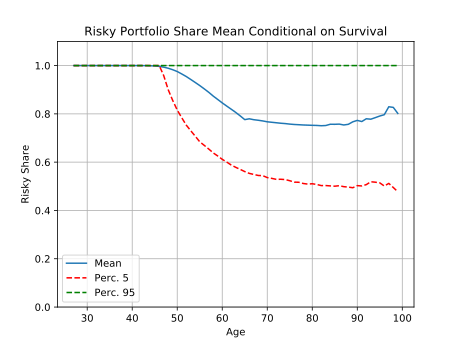
\includegraphics[width=6in]{\econtexRoot/\FigsRaw/RShare_Means}}
	\caption{Risky Portfolio Share Mean Conditional on Survival}
	\label{fig:RShareMean}
\end{figure}
 % Read in the tex to generate the figure

\section{Other results in the original paper}

\subsection{The welfare implications of different allocation rules}

The authors next conduct a welfare analysis of different allocation rules, including popular heuristics. The rules are presented in the Figure \ref{fig:AllocRules}.

\providecommand{\figName}{Allocation-Rules} % Allows generic definition of hypertargets based on title of figure
\providecommand{\figFile}{Alloc_rules} %  and on filename
\hypertarget{\figFile}{}
\hypertarget{\figName}{}
\begin{figure}[]
	\centerline{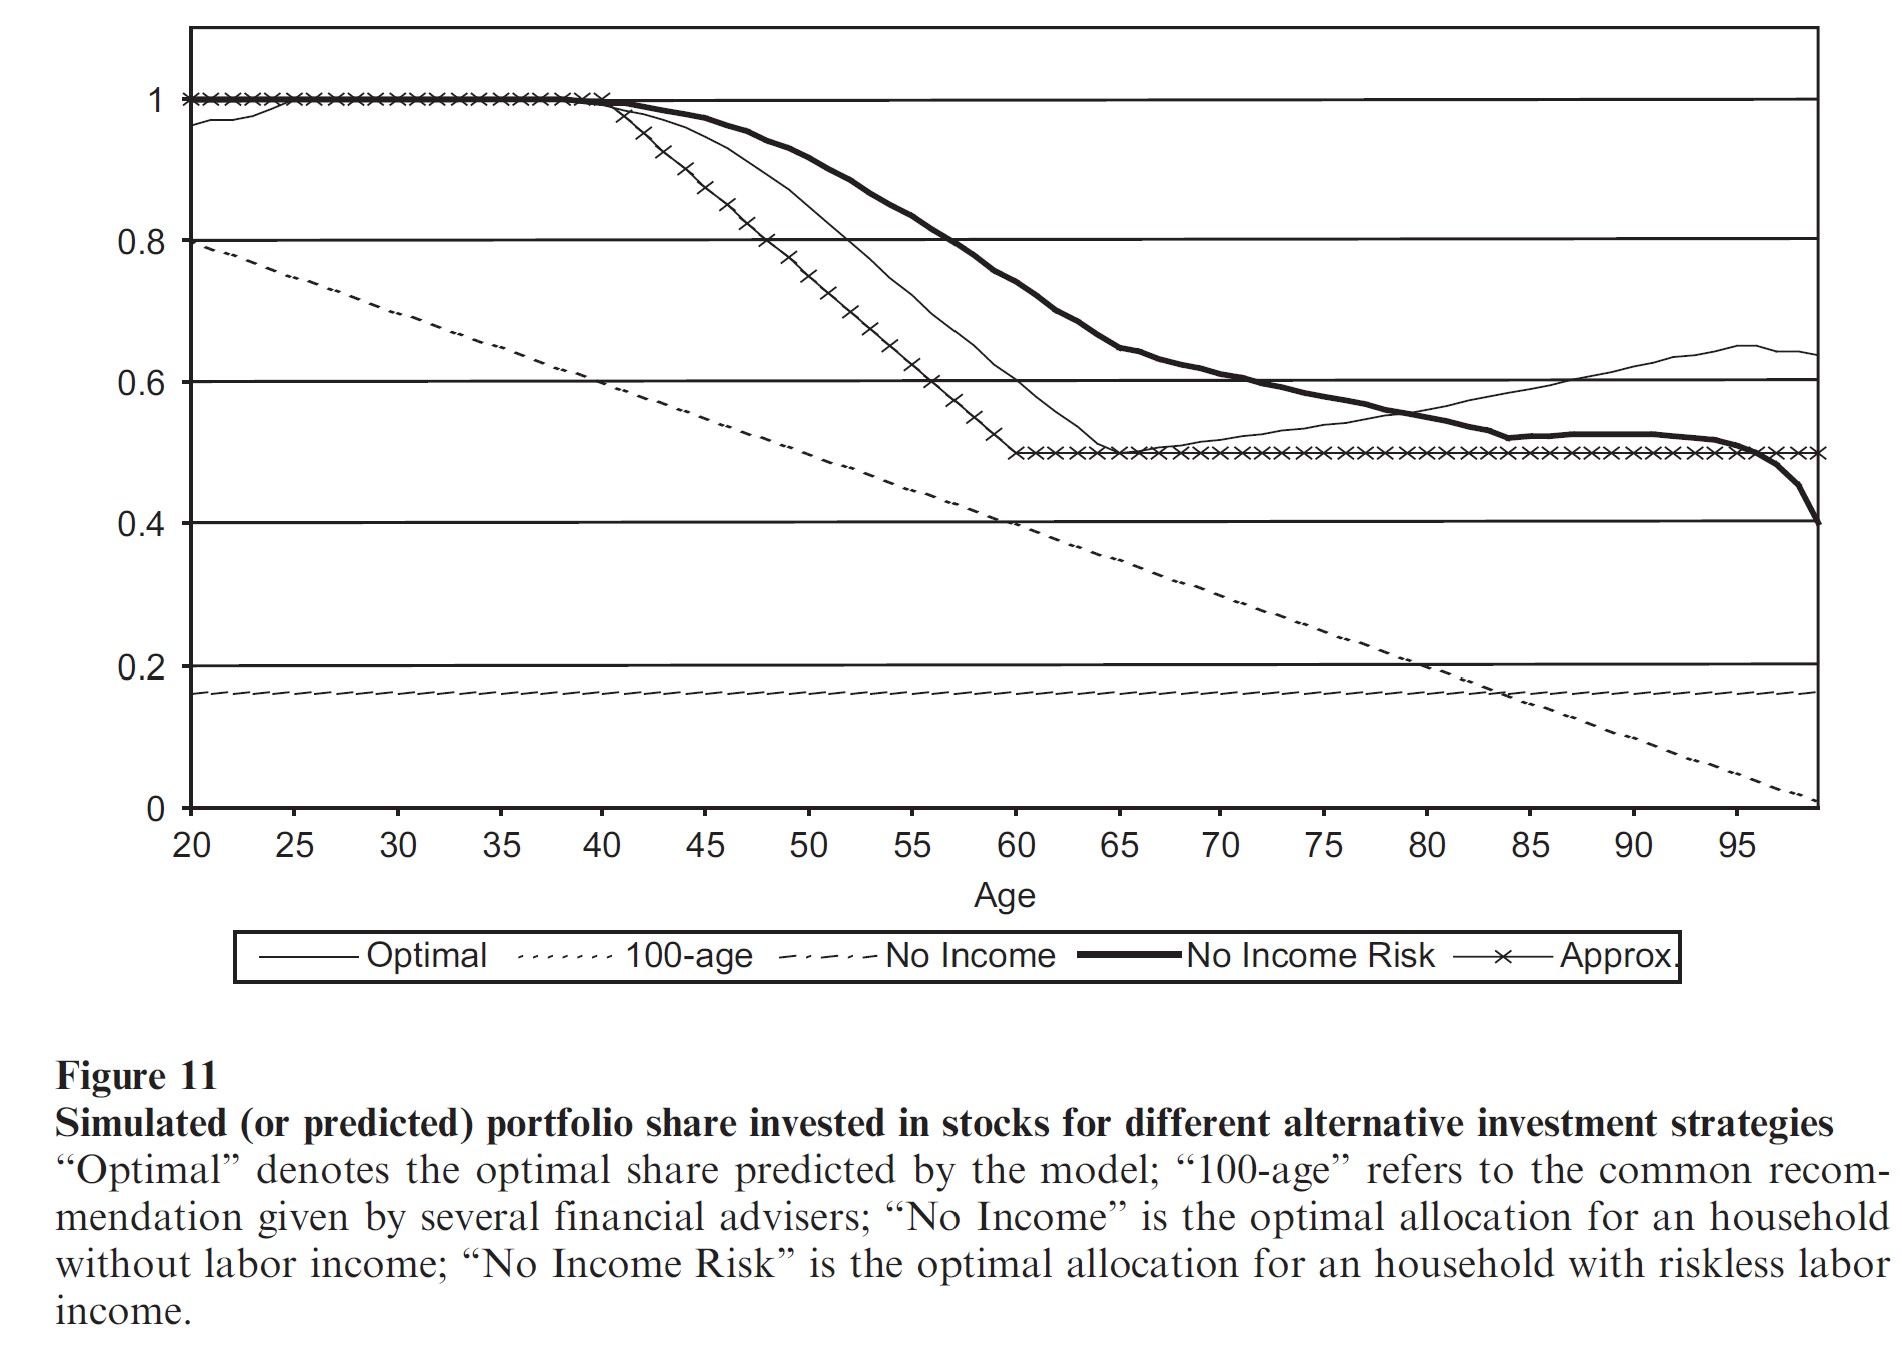
\includegraphics[width=6in]{\econtexRoot/\FigsRaw/Alloc_rules.jpg}}
	\caption{CGM Allocation Rules}
	\label{fig:AllocRules}
\end{figure}
 % Read in the tex to generate the figure

The utility cost of each policy in terms of constant consumption streams with respect to the authors calculated optimal policy function is reported in the next Figure \ref{fig:UtilityCosts}.

\providecommand{\figName}{Utility-Costs} % Allows generic definition of hypertargets based on title of figure
\providecommand{\figFile}{Util_cost} %  and on filename
\hypertarget{\figFile}{}
\hypertarget{\figName}{}
\begin{figure}[]
	\centerline{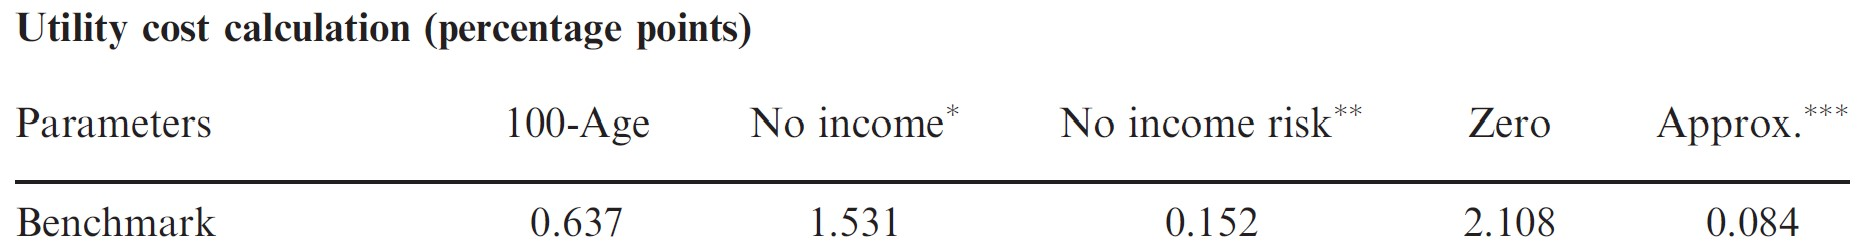
\includegraphics[width=6in]{\econtexRoot/\FigsRaw/Util_cost.jpg}}
	\caption{CGM Utility Costs}
	\label{fig:UtilityCosts}
\end{figure}
 % Read in the tex to generate the figure

Interestingly, the "no-income" column corresponds to the usual portfolio choice result of the optimal share being the quotient of excess returns and risk times relative risk aversion, disregarding labor income. The experiment shows this allocation produces substantial welfare losses.

\subsection{Heterogeneity and sensitivity analysis}

The authors also considered a number of extensions to the baseline model. These are summarized below along with their main conclusions.
\begin{itemize}
	\item Labor income risk: Income risk may vary across employment sectors relative to the baseline model. The authors examine extreme cases for industries that have a large standard deviation and temporary income shocks. While some differences appear across sectors, the results are generally in line with the baseline model.
	\item Disastrous labor income shocks: The authors find that even a small probability of zero labor income lowers the optimal portfolio allocation in stocks, while the qualitative features of the baseline model are preserved.
	\item Uncertain retirement income: The authors consider two types of uncertainty for retirement income; it is stochastic and correlated with current stock market performance and allowing for disastrous labor income draws before retirement. The first extension has results essentially the same as the baseline case. The second leads to more conservative portfolio allocations but is broadly consistent with the baseline model.
	\item Endogenous borrowing constraints: The authors add borrowing to their model by building on credit-market imperfections. They find that the average investor borrows about \$5,000 and are in debt for most of their working life. The agents eventually pay off this debt and save for retirement. Relative to the benchmark model, the investor has put less of their money in their portfolio and arrive at retirement with substantially less wealth. These results are particularly pronounced at the lower end of the income distribution relative to the higher end. Additional details are available in the text.
	\item Bequest motive: The authors introduce a bequest motive into the agent's utility function (i.e., $b>0$). Young investors are more impatient and tend to save less for bequests. As the agent ages, savings increases and is strongest once the agent retires. This leads to effects on the agent's portfolio allocation. Taking a step-back however, these effects are not very large unless $b$ is large.
	\item Educational attainment: The authors generally find that savings are consistent across education groups. They note that for a given age, the importance of future income is increasing with education level. This implies that riskless asset holdings are larger for these households.
	\item Risk aversion and intertemporal substitution: Lowering the level of risk aversion in the model leads to changes in the optimal portfolio allocation and wealth accumulation. Less risk-averse investors accumulate less precautionary savings and invest more in risky assets.
\end{itemize}

\hypertarget{Conclusion}{}
\section{Conclusion}

This article provides a dynamic model with accurate lifetime income profiles in which labor income increases risky asset holdings, as it is seen as a closer substitute of risk-free assets. It finds an optimal risky asset share that decreases in wealth and with age, after middle age. The model is also used to show that ignoring labor income for portfolio allocation can generate substantial welfare losses.

\hypertarget{Puzzles-and-Questions}{}
\section{Puzzles and Questions}\label{sec:Puzzles}
\begin{itemize}
	\item Table 4 in the main text says stock returns are $0.06$. They might 
	mean that the equity premium $\mu$ is $0.06$.
	\item The authors report taking the normalization $v_{i,t} = 1$. However the ranges of their results seem more consistent with $v_{i,t} = 0$ so that $\exp (v_{i,t}) = 1$, which also makes more sense for interpretation.
\end{itemize}

\hypertarget{Robustness Analyses}{}
\section{Robustness Analyses}

Given the differences between our results and the original paper, we did a number of checks to ensure our model was behaving consistently with well-established theoretical results. Specifically we checked:
\begin{itemize}
	\item For an infinitely lived agent with log normal returns, that their optimal portfolio allocation converges to the Campbell-Viceira (2002) approximation to the optimal portfolio share in Merton-Samuelson (1969) model.
	\item For an infinitely lived agent with no labor income that can only invest in a single risky asset, that their marginal propensity to consumer converges to the theoretical MPC of Merton-Samuelson (1969).
	\item For an agent facing no labor income risk, that their consumption patterns precisely match the results from a perfect foresight solution.
\end{itemize}

In all three cases, we verified that our HARK model holds up to these results. More details and specific results are available upon request. 

As the HARK toolkit continues to develop, there are additional sensitivities that we can perform to further check the credibility of our results. Specifically, once human wealth is available in the $\texttt{PortfolioConsumerType}$ class, we can perform the following additional checks, which were kindly suggested by Professor Sylvain Catherine:
\begin{itemize}
	\item Shut down the income risk and remove retirement income. The solution to this new problem are provided by Merton 1971. Basically, you capitalize future earnings as an endowment of risk free asset. Then the equity share should be such that Equity/(Wealth+NPV of Human capital) is the same as the equity share in Merton 1969.
	\item Adding back the permanent income risk and check if the equity share is consistent with Viceira 2001. Viceira tells you something like this: $\pi = \frac{\mu - r}{\gamma \sigma^2_s} + \left(\frac{\mu - r}{\gamma \sigma^2_s} - \beta_{HC} \right) \frac{HC}{W}$, where $\beta_{HC} = \frac{\text{Cov}(r_{HC},r_s)}{\text{Var}(r_s)}$. In the CGM problem it is easy to compute $\beta_{HC}$ because earnings follow a simple random walk. HC is the NPV of human capital, which you can approximate very well by discounting expected earnings by $r+\beta_{HC}*(rm-r)$.
\end{itemize}

\clearpage\vfill\eject

\onlyinsubfile{\bibliography{\econtexRoot/CGMPortfolio-Add}}

\end{document}
